\documentclass{article}
\usepackage{graphicx, tikz-cd, float, titlepic, booktabs} % Required for inserting images
\usepackage{pgfplots}
\pgfplotsset{compat=1.15}
\usepackage{mathrsfs}
\usetikzlibrary{arrows}
\usepackage{amsmath, amssymb, amsthm, amsfonts, siunitx, physics, gensymb}
\AtBeginDocument{\RenewCommandCopy\qty\SI}
\usepackage[version=4]{mhchem}
\usepackage[most,many,breakable]{tcolorbox}
\usepackage{xcolor, fancyhdr, varwidth}
\usepackage[Glenn]{fncychap}
%Options: Sonny, Lenny, Glenn, Conny, Rejne, Bjarne, Bjornstrup
\usepackage{hyperref, cleveref}
\usepackage{icomma, enumitem} %comma as decimal and continue enumerate with [resume]
\usepackage{plimsoll} %use standard state symbol with \stst
\usepackage[danish]{babel}
%%%%%%%%%%%%%%%%%%%%%%%%%%%%%%
% SELF MADE COLORS
%%%%%%%%%%%%%%%%%%%%%%%%%%%%%%
\definecolor{myg}{RGB}{56, 140, 70}
\definecolor{myb}{RGB}{45, 111, 177}
\definecolor{myr}{RGB}{199, 68, 64}
\definecolor{mytheorembg}{HTML}{F2F2F9}
\definecolor{mytheoremfr}{HTML}{00007B}
\definecolor{mylenmabg}{HTML}{FFFAF8}
\definecolor{mylenmafr}{HTML}{983b0f}
\definecolor{mypropbg}{HTML}{f2fbfc}
\definecolor{mypropfr}{HTML}{191971}
\definecolor{myexamplebg}{HTML}{F2FBF8}
\definecolor{myexamplefr}{HTML}{88D6D1}
\definecolor{myexampleti}{HTML}{2A7F7F}
\definecolor{mydefinitbg}{HTML}{E5E5FF}
\definecolor{mydefinitfr}{HTML}{3F3FA3}
\definecolor{notesgreen}{RGB}{0,162,0}
\definecolor{myp}{RGB}{197, 92, 212}
\definecolor{mygr}{HTML}{2C3338}
\definecolor{myred}{RGB}{127,0,0}
\definecolor{myyellow}{RGB}{169,121,69}
\definecolor{myexercisebg}{HTML}{F2FBF8}
\definecolor{myexercisefg}{HTML}{88D6D1}
%%%%%%%%%%%%%%%%%%%%%%%%%%%%%%%%%%%%%%%%%%%%%%%%%%%%%%%%%%%%%%%%%%%%%%
% Box environments for theorems and problems
%%%%%%%%%%%%%%%%%%%%%%%%%%%%%%%%%%%%%%%%%%%%%%%%%%%%%%%%%%%%%%%%%%%%%
\setlength{\parindent}{1cm}
%================================
% Question BOX
%================================
\makeatletter
\newtcbtheorem{question}{Opgave}{enhanced,
	breakable,
	colback=white,
	colframe=myb!80!black,
	attach boxed title to top left={yshift*=-\tcboxedtitleheight},
	fonttitle=\bfseries,
	title={#2},
	boxed title size=title,
	boxed title style={%
			sharp corners,
			rounded corners=northwest,
			colback=tcbcolframe,
			boxrule=0pt,
		},
	underlay boxed title={%
			\path[fill=tcbcolframe] (title.south west)--(title.south east)
			to[out=0, in=180] ([xshift=5mm]title.east)--
			(title.center-|frame.east)
			[rounded corners=\kvtcb@arc] |-
			(frame.north) -| cycle;
		},
	#1
}{def}
\makeatother
%================================
% DEFINITION BOX
%================================

\newtcbtheorem[]{Definition}{Definition}{enhanced,
	before skip=2mm,after skip=2mm, colback=red!5,colframe=red!80!black,boxrule=0.5mm,
	attach boxed title to top left={xshift=1cm,yshift*=1mm-\tcboxedtitleheight}, varwidth boxed title*=-3cm,
	boxed title style={frame code={
					\path[fill=tcbcolback]
					([yshift=-1mm,xshift=-1mm]frame.north west)
					arc[start angle=0,end angle=180,radius=1mm]
					([yshift=-1mm,xshift=1mm]frame.north east)
					arc[start angle=180,end angle=0,radius=1mm];
					\path[left color=tcbcolback!60!black,right color=tcbcolback!60!black,
						middle color=tcbcolback!80!black]
					([xshift=-2mm]frame.north west) -- ([xshift=2mm]frame.north east)
					[rounded corners=1mm]-- ([xshift=1mm,yshift=-1mm]frame.north east)
					-- (frame.south east) -- (frame.south west)
					-- ([xshift=-1mm,yshift=-1mm]frame.north west)
					[sharp corners]-- cycle;
				},interior engine=empty,
		},
	fonttitle=\bfseries,
	title={#2},#1}{def}
\newtcbtheorem[]{definition}{Definition}{enhanced,
	before skip=2mm,after skip=2mm, colback=red!5,colframe=red!80!black,boxrule=0.5mm,
	attach boxed title to top left={xshift=1cm,yshift*=1mm-\tcboxedtitleheight}, varwidth boxed title*=-3cm,
	boxed title style={frame code={
					\path[fill=tcbcolback]
					([yshift=-1mm,xshift=-1mm]frame.north west)
					arc[start angle=0,end angle=180,radius=1mm]
					([yshift=-1mm,xshift=1mm]frame.north east)
					arc[start angle=180,end angle=0,radius=1mm];
					\path[left color=tcbcolback!60!black,right color=tcbcolback!60!black,
						middle color=tcbcolback!80!black]
					([xshift=-2mm]frame.north west) -- ([xshift=2mm]frame.north east)
					[rounded corners=1mm]-- ([xshift=1mm,yshift=-1mm]frame.north east)
					-- (frame.south east) -- (frame.south west)
					-- ([xshift=-1mm,yshift=-1mm]frame.north west)
					[sharp corners]-- cycle;
				},interior engine=empty,
		},
	fonttitle=\bfseries,
	title={#2},#1}{def}

\newtcbtheorem{theo}%
    {Theorem}{}{theorem}
\newtcolorbox{prob}[1]{colback=red!5!white,colframe=red!50!black,fonttitle=\bfseries,title={#1}}
%================================
% NOTE BOX
%================================

\usetikzlibrary{arrows,calc,shadows.blur}
\tcbuselibrary{skins}
\newtcolorbox{note}[1][]{%
	enhanced jigsaw,
	colback=gray!20!white,%
	colframe=gray!80!black,
	size=small,
	boxrule=1pt,
	title=\textbf{Note:},
	halign title=flush center,
	coltitle=black,
	breakable,
	drop shadow=black!50!white,
	attach boxed title to top left={xshift=1cm,yshift=-\tcboxedtitleheight/2,yshifttext=-\tcboxedtitleheight/2},
	minipage boxed title=1.5cm,
	boxed title style={%
			colback=white,
			size=fbox,
			boxrule=1pt,
			boxsep=2pt,
			underlay={%
					\coordinate (dotA) at ($(interior.west) + (-0.5pt,0)$);
					\coordinate (dotB) at ($(interior.east) + (0.5pt,0)$);
					\begin{scope}
						\clip (interior.north west) rectangle ([xshift=3ex]interior.east);
						\filldraw [white, blur shadow={shadow opacity=60, shadow yshift=-.75ex}, rounded corners=2pt] (interior.north west) rectangle (interior.south east);
					\end{scope}
					\begin{scope}[gray!80!black]
						\fill (dotA) circle (2pt);
						\fill (dotB) circle (2pt);
					\end{scope}
				},
		},
	#1,
}
%================================
% EXAMPLE BOX
%================================
\newtcbtheorem[number within=section]{Example}{Example}
{%
	colback = myexamplebg
	,breakable
	,colframe = myexamplefr
	,coltitle = myexampleti
	,boxrule = 1pt
	,sharp corners
	,detach title
	,before upper=\tcbtitle\par\smallskip
	,fonttitle = \bfseries
	,description font = \mdseries
	,separator sign none
	,description delimiters parenthesis
}
{ex}
%================================
% THEOREM BOX
%================================

\tcbuselibrary{theorems,skins,hooks}
\newtcbtheorem[number within=section]{Theorem}{Theorem}
{%
	enhanced,
	breakable,
	colback = mytheorembg,
	frame hidden,
	boxrule = 0sp,
	borderline west = {2pt}{0pt}{mytheoremfr},
	sharp corners,
	detach title,
	before upper = \tcbtitle\par\smallskip,
	coltitle = mytheoremfr,
	fonttitle = \bfseries\sffamily,
	description font = \mdseries,
	separator sign none,
	segmentation style={solid, mytheoremfr},
}
{th}

%%%%%%%%%%%%%%%%%%%%%%%%%%%%%%%%%%%%%%%%%%%%%%%%%%%%%%%%%%%%%%%%%
% SELF MADE COMMANDS
%%%%%%%%%%%%%%%%%%%%%%%%%%%%%%
\newcommand{\sol}{\setlength{\parindent}{0cm}\textbf{\textit{Løsning:}}\setlength{\parindent}{1cm}}
%%%%%%%%%%%%%%%%%%%%%%%%%%%%%%%%%
\usepackage[tmargin=2cm,rmargin=1in,lmargin=1in,margin=0.85in,bmargin=2cm,footskip=.2in]{geometry}\pagestyle{fancy}
\lhead{Minrui Kevin Zhou 3.b}
\rhead{Matprøve 2}

\title{Matprøve 2\\
{\Large \textbf{3.b mat A}}}
\author{Kevin Zhou}
\date{\today}

\begin{document}
\maketitle
\newpage
\begin{question}{}{}
To funktioner $f$ og $g$ er givet ved
\[
f(x)= -x^2+3x+5
\] 
og 
\[
g(x)= 5.
\] 
Grafen for $f$ og grafen for $g$ afgrænser et område $M$ i første kvadrant.
\begin{itemize}
  \item[a.] Bestem arealet af $M$.
  \item[b.] Bestem rumfanget af det omdrejningslegeme, som fremkommer, når $M$ drejes $360 \degree $ om førsteaksen. 
\end{itemize}
\end{question}
\sol \\
\textbf{a.}
Vi finder først de $x$-værdier, hvor graferne for $f$ og $g$ skærer hinanden.
\begin{equation*}
\begin{split}
  f(x)= g(x)&\iff -x^2+3x+5=5\\
  &\iff x(-x+3)=0\\
  &\iff x=0 \lor x=3
\end{split}
\end{equation*}
Siden både $f$ og $g$ er kontinuerte og $1 \in [0;3]$ samt at $f(1)=7>g(1)=5$, så må der gælde, at
\[
x \in [0;3] \implies f(x) \geq g(x)
\] 
Altså må arealet af $M$ være
\begin{equation*}
\begin{split}
  A(M)&=\int_{0}^{3} \left(f(x)-g(x)\right)  \,dx \\
  &=\int_{0}^{3} \left(-x^2+3x+5-5\right)  \,dx \\
  &=\int_{0}^{3} \left( -x^2+3x\right) \,dx \\
  &=\left[-\frac{1}{3}x^3 + \frac{3}{2}x^2\right]_{0}^{3}\\
  &=-3^2+\frac{3^3}{2}\\
  &=\frac{27}{2}-9\\
  &=\frac{9}{2}
\end{split}
\end{equation*}
Arealet af $M$ er altså $\frac{9}{2}$. \\[1ex]
\textbf{b.}
Rumfanget af det hule omdrejningslegeme må være
\begin{equation*}
\begin{split}
  V&= \pi \int_{0}^{3} \left(f(x)^2-g(x)^2\right)  \,dx \\
  &=\pi \int_{0}^{3} ((-x^2+3x+5)^2-5^2) \,dx \\
  &=\frac{531}{10} \pi 
\end{split}
\end{equation*}
Der er løst med CAS (se \cref{fig:CAS}).
Altså er rumfanget af det omdrejningslegeme, som fremkommer, når $M$ drejes $360 \degree $ om førsteaksen $\frac{531}{10} \pi $.
\begin{figure}[H]
\begin{center}
  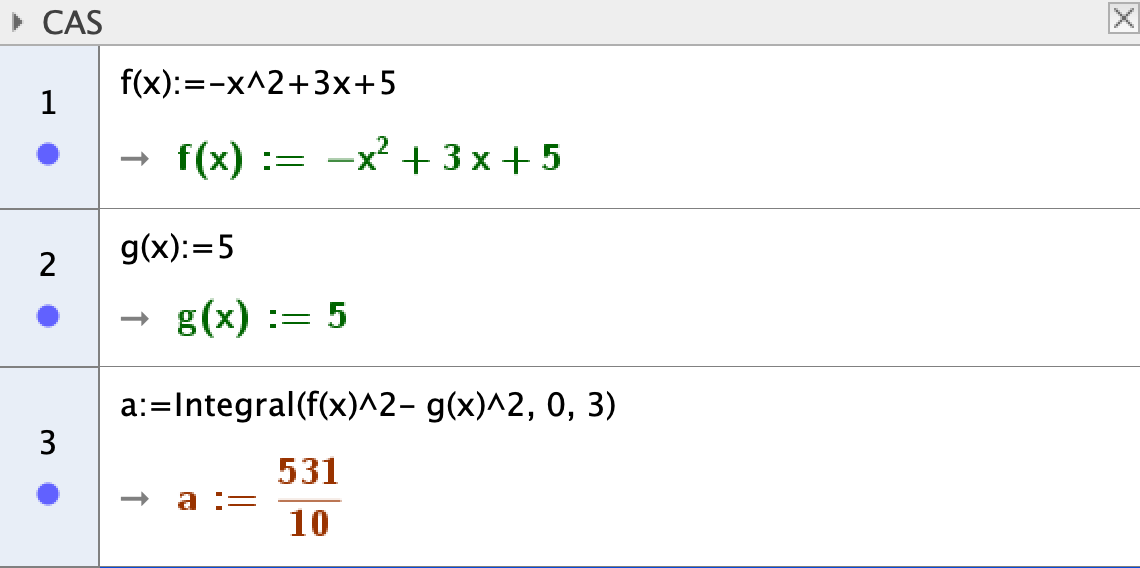
\includegraphics[width=\textwidth]{CAS.png}
\end{center}
\caption{Integralet løst med CAS}
\label{fig:CAS}
\end{figure}
\begin{question}{}{}
  I en model er længden $L$ af en torsk (målt i cm) en funktion af torskens alder $t$ (målt i år), og det antages, at differentialligning gælder:
  \[
  \dv{L}{t}=k \cdot \left(150-L\right), 
  \] 
  hvor $k$ er en konstant. 
Det oplyses, at til tiden $t = 0$ er torskens længde 1 cm, og til tiden $t = 1$ er torskens længden 15 cm.
\begin{itemize}
  \item[a.] Bestem $L$ som funktion af $t$.
  \item[b.] Bestem aldersintervallet for de torsk, som er mellem $50 \;\unit{cm} $ og $100 \;\unit{cm} $ lange ifølge modellen. 
\end{itemize}
\end{question}
\sol \\
\textbf{a.}
Vi omskriver differentialligningen 
\begin{equation*}
\begin{split}
  \dv{L}{t}=k \cdot \left(150-L\right) \iff \dv{L}{t}=150k - kL
\end{split}
\end{equation*}
Siden der for ligningen $y'=b-a \cdot y$ gælder, at den har løsningerne $y=\frac{b}{a}+c \cdot e^{-ax} $, så må løsninger for $L$ være af formen
\begin{equation*}
\begin{split}
  L(t)&=\frac{150k}{k}+c \cdot e^{-kx}\\
  &=150 + c \cdot e^{-kx} 
\end{split}
\end{equation*}
Siden $L(0)=1$, så har vi 
\begin{equation*}
\begin{split}
  L(0)=1 &\iff 150 + c \cdot e^{-k \cdot 0} =1\\
  &\iff 150 + c=1\\
  &\iff c=-149
\end{split}
\end{equation*}
Da vi ved at $L(1)=15$, så kan vi også finde $k$.
\begin{equation*}
\begin{split}
  L(1)=15 &\iff 150 -149 \cdot e^{-k \cdot 1} =15\\
  &\iff e^{-k} =\frac{135}{149}\\
  &\iff k=-\ln\left(\frac{135}{149}\right) 
\end{split}
\end{equation*}
$L$ som funktion af $t$ er altså 
\begin{equation*}
\begin{split}
  L(t)=150-149 \cdot e^{\ln\left(\frac{135}{149}\right) \cdot x} 
\end{split}
\end{equation*}
\textbf{b.}
Aldersintervallet findes ved at løse ligningen 
\[
50<L(t)<100 \implies 4,04<t<11,07 
\] 
der løses med CAS (se \cref{fig:CAS2}).
Aldersintervallet er altså $t \in ]4,04;11,07[$.

\begin{figure}[H]
\begin{center}
  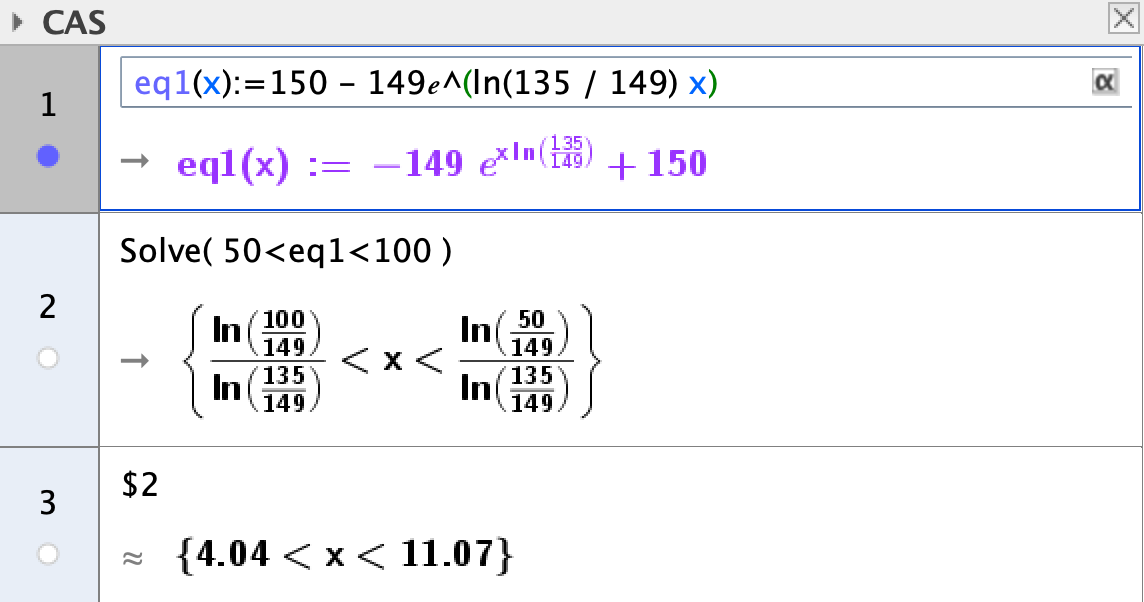
\includegraphics[width=\textwidth]{CAS2.png}
\end{center}
\caption{Ligningen løses med CAS}
\label{fig:CAS2}
\end{figure}

\end{document}
